\documentclass[11pt,a4]{article}

\parindent=0pt
\parskip=3pt

\setlength{\paperheight}{29.5cm}
\setlength{\paperwidth}{21.2cm}

%\setlength{\voffset}{-2.0cm}
\setlength{\headheight}{0cm}
\setlength{\headsep}{0cm}
\setlength{\textheight}{23.7cm}
\setlength{\textwidth}{16cm}
\setlength{\oddsidemargin}{0cm}
\setlength{\evensidemargin}{0cm}
\setlength{\topmargin}{0cm}
\setlength{\topskip}{0cm}

\catcode`\"=\active \let"=\"
\let\3=\ss

\usepackage[latin9]{inputenc}

\usepackage[sort]{natbib}
\bibpunct{(}{)}{,}{a}{}{,}

\usepackage{amsmath}
\usepackage{amssymb}

%\usepackage[squaren]{SIunits}
\usepackage{graphicx}

%----------------------------------------------------------------------------
%---- Farben und Macros zur Textmarkierung ----------------------------------
%----------------------------------------------------------------------------
\usepackage{color}
\definecolor{light}{gray}{0.50}
\definecolor{heavy}{gray}{0.35}
\definecolor{black}{gray}{0.0}
\definecolor{dgreen}{rgb}{0.0,0.7,0}
\definecolor{dred}{rgb}{0.9959,0,0}
\definecolor{green}{rgb}{0.0,0.99599,0.0}
\definecolor{purple}{rgb}{0.6,0.0,0.4}

\newcommand{\red}[1]{\textcolor{dred}{#1}}
\newcommand{\green}[1]{\textcolor{green}{#1}}
\newcommand{\dgreen}[1]{\textcolor{dgreen}{#1}}
\newcommand{\purple}[1]{\textcolor{purple}{#1}}
\newcommand{\blue}[1]{\textcolor{blue}{#1}}
\newcommand{\black}[1]{\textcolor{black}{#1}}
\newcommand{\grey}[1]{\textcolor{heavy}{#1}}
\newcommand{\lightgrey}[1]{\textcolor{light}{#1}}

%----------------------------------------------------------------------------
%---- Kommentare ------------------------------------------------------------
%----------------------------------------------------------------------------

\newcommand{\klein}[1]{\textcolor{blue}{#1}}
\newcounter{kleincommentno}
\setcounter{kleincommentno}{1}
\newcommand{\kleincomment}[1]{{\small\bfseries\textcolor{blue}{ {\small\bfseries${}^{[\arabic{kleincommentno}]}$}}%
\marginpar{\textcolor{blue}{{\small{\bfseries[\arabic{kleincommentno}]}\ \small #1}}\addtocounter{kleincommentno}{1}}}}

\newcommand{\benacchio}[1]{\textcolor{red}{#1}}
\newcounter{benacchiocommentno}
\setcounter{benacchiocommentno}{1}
\newcommand{\benacchiocomment}[1]{{\small\bfseries\textcolor{red}{ {\small\bfseries${}^{[\arabic{benacchiocommentno}]}$}}%
\marginpar{\textcolor{red}{{\small{\bfseries[\arabic{benacchiocommentno}]}\ \small #1}}\addtocounter{benacchiocommentno}{1}}}}

%----------------------------------------------------------------------------
%---- Eigene Macros ---------------------------------------------------------
%----------------------------------------------------------------------------
\newcommand{\hsc}{h_{\rm sc}}
\newcommand{\order}[1]{^{(#1)}}
\let\dss=\displaystyle

\renewcommand{\vector}[1]{\relax\ifmmode\mathchoice
{\mbox{\boldmath$\displaystyle#1$}}
{\mbox{\boldmath$\displaystyle#1$}}
{\mbox{\boldmath$\scriptstyle#1$}}
{\mbox{\boldmath$\scriptscriptstyle#1$}}\else
\hbox{\boldmath$\textstyle#1$}\fi}

\newcommand{\eq}[1]{(\ref{#1})}

\newcommand{\cbar}{\overline{c}}
\newcommand{\thetabar}{\overline{\theta}}
\newcommand{\thetatilde}{\widetilde{\theta}}

\newcommand{\vk}{\vector{k}}
\newcommand{\vu}{\vector{u}}
\newcommand{\vv}{\vector{v}}
\newcommand{\vx}{\vector{x}}

\newcommand{\ubar}{\overline{u}}
\newcommand{\vbar}{\overline{v}}


\newcommand{\advection}[1]{\mathcal{A}\left[#1\right]}
\newcommand{\advectionNum}[1]{\widetilde{\mathcal{A}}\left[#1\right]}
\newcommand{\rhs}[1]{\mathcal{R}\left[#1\right]}
\newcommand{\source}[1]{S\left(#1\right)}
\newcommand{\Id}{{\rm Id}}

\newcommand{\pprime}{p'}
\newcommand{\half}{\frac{1}{2}}
\newcommand{\quart}{\frac{1}{4}}
\newcommand{\eightth}{\frac{1}{8}}

\newcommand{\ie}{\emph{i.e.}}

\newcommand{\Nscsq}{N^2_{sc}}

% ===========================================================================
% ===========================================================================
% ===========================================================================
% ===========================================================================

\title{Notes on semi-implicit time stepping, blended models, etc.}
\author{T.~Benacchio, MetOffice, Exeter, UK\\ 
        R.~Klein, Mathematics \& Informatics, Freie Universit\"at Berlin}

\begin{document}

\maketitle

% ===========================================================================
% ===========================================================================
% ===========================================================================

\section*{ToDo}

\paragraph{January 19, 2018 (additions of January 25, 2018):}
%
\begin{itemize}
\item get compressible version going as the long-wave hydrostatic GW test
      might involve a compressibility influence \\
      (Set aside as long as I have no psinc version really running.)
\item re-implement Runge-Kutta time integrator for the explicit part\\
      (Set aside.)
\item Move 1st projection to the half-time level of the second-order RK-scheme\\
      (Will do so now, but keep the split/MUSCL scheme for now.)
\item Can I invent a scheme that explicitly advects $\tilde\theta$ instead of
      full theta and thus allows me to control up-down symmetry better?\\
      (Part of my next move.)
\end{itemize}
%

\paragraph{January 25, 2018: New scheme}

The key difficulty with my approach so far seems to be that the time 
semi-implicit integration is not consistently carried through the scheme. 
I am using the ingredients of the implicit midpoint rule in formulating
and stabilizing the advective fluxes, yet I am so far not fully evaluating
the implicit terms at the mid-time level. This would entail solving the 
pressure equation right there and accounting for the pressure gradients
in correcting the advective fluxes also. This I am going to fix with the
following strategy:
%
\begin{enumerate}
\item \label{it:LeadingSplitStep}
      Split-step advection forward cycle, including separated treatment 
      of $\tilde\theta$, with the contribution from the background 
      stratification taken out and shifted to the flux correction part.
      Density transport is carried along as part of the compressible 
      advection scheme. (See ``Options''�below.) 
\item Advective flux correction including a correction that takes the 
      split-step advection fluxes out and replaces them with fluxes 
      computed afresh from the data obtained after 
      step~\ref{it:LeadingSplitStep}. Only now will the advection of the
      background be handled and added to $\tilde\theta$.
\item Implicit momentum correction corresponding to ``second projection''
      in our previous work. (See ``Options''.)
\item Concluding advection split step. 
\end{enumerate}
%

Options:
%
\begin{itemize}
\item Options for compressible advection:
  \begin{enumerate}
  \item Standard procedure based on $(\rho, \rho\vv, P)$. The split into
        an additional transport scheme for $\tilde\rho = (P\tilde\theta)$
        may introduce a breach of mass continuity if $\rho$ is replaced 
        with the result of the decomposed step after the fact. It might
        be sufficient, though, to just use the split-version as an auxiliary
        means of formulating balanced fluxes. 
  \item Switch to formulating advection in terms of $(P\tilde\theta, P\vv, P)$. 
        In this approach, we likely don't even have to invoke an additional
        variable.  
  \end{enumerate}
\item Options for second projection / balanced momentum update
  \begin{enumerate}
  \item Treat implicit advection of background stratification as auxiliary
        calculation.
  \item Use ``single projection only'' approach developed earlier and 
        implemented under \\ ``NODAL\_PROJECTION\_ONLY'' in RKLM code variant.
  \end{enumerate}
\end{itemize}
%


% ===========================================================================
% ===========================================================================
% ===========================================================================

\section{Introduction}
\label{sec:Intro}

Previous attempts at implementing the semi-implicit time discretization
strategy as explicated in T.~Benacchio's thesis have not allowed us to
go to time steps larger than $N\Delta t$, where $N$ is the Brunt-V�is�l�
frequency and $\Delta t$ the time step. It seems that it is necessary to
split advection of potential temperature, $\theta$, into that of its
large-scale horizontal mean, $\thetabar$, and deviations, $\thetatilde$,
from it. Advection of the former becomes part of the (quasi-)linearized
implicity system and that of the latter remains part of the explicit
advection step. This corresponds to the usual practice of subtracting
out a background profile of $\theta$ at the differential equation level. 
A dynamically evolving and horizontally non-homogeneous background can be 
thought of in terms of a multiscale/multigrid strategy, but we leave this
for later. 

The time stepping strategy to be described here follows closely that
described by P.~Smolarkiewicz in a series of papers, see, e.g., 
\citep{SmolarkiewiczMargolin1998,SmolarkiewiczEtAl2014}.

% ===========================================================================
% ===========================================================================
% ===========================================================================

\section{Getting rid of the first (MAC) projection}
\label{sec:NoFirstProjection}

% ===========================================================================
% ===========================================================================

\subsection{Node- and cell-centered divergences}
\label{ssec:NodeCellDiv}

Currently, our scheme invokes two sequential projections / Helmholtz-solves
to realize consistent divergence of the advective fluxes $P\vv$. The first
fixes the actual flux divergence employed in discretizing the advection 
terms, the second makes sure that the cell centered velocities are compatible
with the respective constraint as well.

Two elliptic solves are expensive, so the question naturally arises as to 
whether there is a way to eliminate one of them. Here is a suggestion for
how to achieve this without losing second-order accuracy. This suggestion
is partially inspired by the time stepping and spatial discretization 
strategy of Piotr Smolarkiewicz' EULAG code 
\citep[see, e.g.,][]{SmolarkiewiczMargolin1998}. 

The key observation can be explained on the basis of 
Fig.~\ref{fig:Divergence}. 
%
\begin{figure}[htbp]
\begin{center}
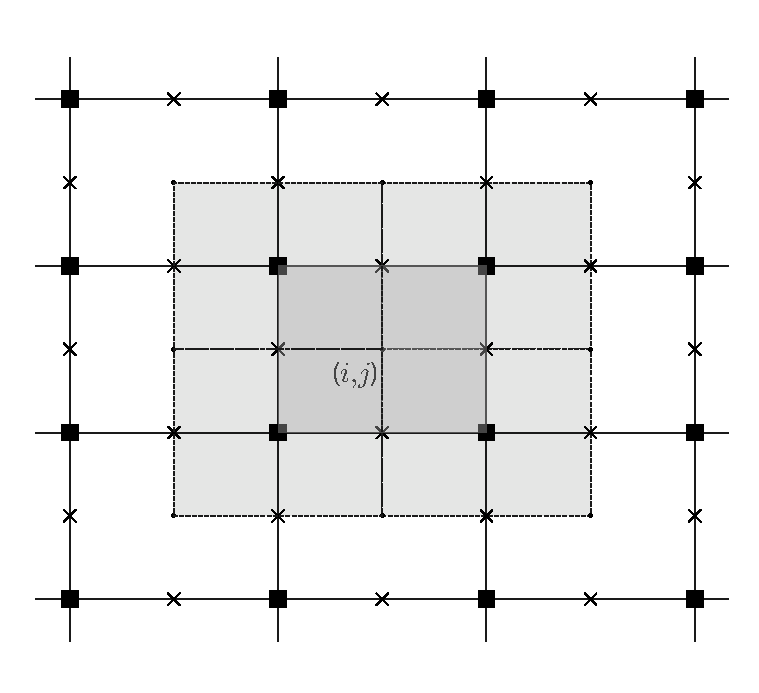
\includegraphics[width=0.5\textwidth]{Graphics/PrimaryAndDualGrid}
\caption{Arrangement of primary and dual cells surrounding a reference cell 
$(i,j)$ on a cartesian 2D mesh.}
\label{fig:Divergence}
\end{center}
\end{figure}
%
The ``second projection'' in the current setting involves a discrete
divergence for each node (filled squares in Fig.~\ref{fig:Divergence}), 
\ie, for some vector field $\vv = (u,v)^t$ we have
%
\begin{equation}
\widetilde{\left(\nabla\cdot\vv\right)}_{i+\half,j+\half}
= 
\frac{(u_{i+1,j}+u_{i+1,j+1}) - (u_{i,j}+u_{i,j+1})}{2\Delta x}
+
\frac{(v_{i,j+1}+v_{i+1,j+1}) - (v_{i+1,j}+v_{i,j})}{2\Delta y}\,.
\end{equation}
%
Now we observe that averaging these divergences over the four dual cells
that overlap with cell $(i,j)$, we obtain a valid divergence discretization
for that cell, 
%
\begin{equation}
\quart\left(
  \widetilde{\left(\nabla\cdot\vv\right)}_{i+\half,j+\half}
+ \widetilde{\left(\nabla\cdot\vv\right)}_{i-\half,j+\half}
+ \widetilde{\left(\nabla\cdot\vv\right)}_{i-\half,j-\half}
+ \widetilde{\left(\nabla\cdot\vv\right)}_{i+\half,j-\half}
\right)
=
\overline{\left(\nabla\cdot\vv\right)}_{i,j}
\end{equation}
%
where
%
\begin{equation}
\overline{\left(\nabla\cdot\vv\right)}_{i,j} 
=
\frac{\ubar_{i+\half,j} - \ubar_{i-\half,j}}{\Delta x}
+
\frac{\vbar_{i,j+\half} - \vbar_{i,j-\half}}{\Delta y}
\end{equation}
%
with the averaged primary cell interface velocities
%
\begin{equation}\label{eq:NodeToFaceAveraging}
\begin{array}{rcl}
\dss \ubar_{i+\half,j}
  & = 
    & \dss
      \eightth
        \left(\left[u_{i+1,j+1} + 2u_{i+1,j} + u_{i+1,j-1}\right] + 
              \left[u_{i,j+1}   + 2u_{i,j}   + u_{i,j-1}  \right]\rule{0pt}{12pt}
        \right)
      \\[10pt]
\dss \vbar_{i,j+\half}
  & = 
    & \dss
      \eightth
        \left(\left[v_{i+1,j+1} + 2v_{i,j+1} + v_{i-1,j+1}\right] + 
              \left[v_{i+1,j}   + 2v_{i,j}   + v_{i-1,j}  \right]\rule{0pt}{12pt}
        \right)\,.
\end{array}
\end{equation}
%
We conclude that from the dual cell discrete divergence we can readily 
construct a compatible primary cell discrete divergence in conseration form.
This is the key in replacing the MAC-projection of the scheme. 

% ===========================================================================
% ===========================================================================

\subsection{Outline of modified divergence control}
\label{ssec:OutlineDivControl}

The advecting fluxes $(P\vv)^{n+\half}$ should ideally be determined
using the implicit trapezoidal rule so that
%
\begin{equation}
(P\vv)^{n+\half} = \half \left((P\vv)^{n} + (P\vv)^{n+1}\right)\,.
\end{equation}
%

\begin{enumerate}

\item
Store the cellface advective fluxes at time level $n$ based on 
\eq{eq:NodeToFaceAveraging} in two separate fields. The first is to
keep this quantity, the second is to be modified in the course of 
a time step to bring it to the new time level. Let us denote these
fields by $(P\vv)^{n}$ and $(P\vv)^{n+\xi}$

\item 
Run the explicit predictor as before with the only exception of how the
advective fluxes are determined in the flux function. Instead of directly
letting, e.g., in the first $x$-step, 
%
\begin{equation}
(Pu)_{i+\half,j}^{n+\xi_1} 
= \half \left((Pu)_{i^+,j}^{n+\xi_1} + (Pu)_{[i+1]^{-},j}^{n+\xi_1}\right)
\end{equation}
%
with $[\cdot]_{i^{+},j}$ denoting reconstructed states at the split-step
half time level at the right edge of primary cell $(i,j)$, we let
%
\begin{equation}
(Pu)_{i+\half,j}^{n+\xi_{m+1}} 
= (Pu)_{i+\half,j}^{n+\xi_{m}}
+ 
\widetilde{\Delta \left(Pu\right)}_{i+\half,j}^{n+\xi_{m+1}}
\end{equation}
%
with the increment obtained from the local MUSCL-type reconstruction as
%
\begin{equation}
\begin{array}{rcl}
\dss \widetilde{\Delta \left(Pu\right)}_{i+\half,j}^{n+\xi_{m+1}} 
  & = 
    & \dss \quart \left((Pu)_{i^+,j} + (Pu)_{i^-,j} 
             + (Pu)_{[i+1]^{-},j} + (Pu)_{[i+1]^{+},j}\right)^{n+\xi_{m+1}}
      \\[10pt]
  & 
    & \dss - \half \left((Pu)_{i,j} + (Pu)_{[i+1],j}\right)^{n+\xi_m}
\end{array}
\end{equation}
%

\item
Once the predictor is done the advective fluxes in the second auxiliary
field have been updated provisionally using the explicit scheme to
time level $t^{n+\half}$, which are labelled 
%
\begin{equation}
(Pu)_{i+\half,j}^{n+\half,\nu}, \quad (Pu)_{i,j+\half}^{n+\half,\nu}\,.
\end{equation}
% 
To start the divergence correction iterations, 
let $\nu = 0$.

\item 
Next we want a divergence-controlled velocity field at $t^{n+1}$. To this
end, run the second projection for the cell-centered fields. From the 
corrected $(P\vv)_{i,j}^{n+1,\nu}$ field, compute advecting fluxes at
the cell faces using \eq{eq:NodeToFaceAveraging}. This generates the fields
%
\begin{equation}
(Pu)_{i+\half,j}^{n+1,\nu}, \quad (Pu)_{i,j+\half}^{n+1,\nu}\,.
\end{equation}
% 

\item 
From these, and the old time level advective fluxes we obtain the 
next iterate for the half-time advective fluxes
%
\begin{equation}
(P\vv)^{n+\half,\nu+1} 
= 
\half \left((P\vv)^{n+1,\nu} + (P\vv)^{n} \right)
\end{equation}
% 

\item
The $\nu$th correction cycle is completed by running the advection
correction based on the advective flux increments
%
\begin{equation}
\Delta (P\vv)^{n+\half,\nu} = (P\vv)^{n+\half,\nu+1} - (P\vv)^{n+\half,\nu}\,. 
\end{equation}
% 

\item 
Check convergence and either continue the iteration or stop.

\item

\item
Run the scheme as before up until the first projection would be invoked, 
except that the advecting fluxes are now computed using the averaging 
formulae in \eq{eq:NodeToFaceAveraging}. Also, the effective advective
fluxes over the entire advection cycle (be it computed via OpSplit or
RK) are to be monitored. This yields advective fluxes 
$(Pu)_{i+\half,j}^{\nu,n+\half}$ and $(Pv)_{i,j+\half}^{\nu,n+\half}$
for $\nu = 0$.

\item\label{eq:Run2ndProj}
Run the node-centered projection to obtain the next iterate of the 
divergence corrected cell-centered velocities. Compute first iterate target 
cell interface advective fluxes using \eq{eq:NodeToFaceAveraging}, 
$(Pu)_{i+\half,j}^{\nu+1,n+\half}$ and $(Pv)_{i,j+\half}^{\nu+1,n+\half}$. 

\item
Correct advection results based on the advecting flux differences 
$(Pu)_{i+\half,j}^{\nu+1,n+\half} - (Pu)_{i+\half,j}^{\nu,n+\half}$
and 
$(Pv)_{i,j+\half}^{\nu+1,n+\half} - (Pv)_{i,j+\half}^{\nu,n+\half}$.

\item If 
$\parallel (P\vv)^{\nu+1,n+\half} - (P\vv)^{\nu,n+\half}\parallel \ 
\geq {\rm tol}$ \ 
return to step \ref{eq:Run2ndProj}, else we are done.

\end{enumerate}


% ===========================================================================
% ===========================================================================
% ===========================================================================

\section{The time stepping strategy}
\label{sec:TimeStepping}

Let $U$ denote our vector of unknowns, which are generally conserved 
quantities in the standard sense, except maybe for the energy variable.
Here we use $P = \rho\theta$ for energy as in 
\citep{KleinTCFD2009,BenacchioEtAl2014}, where $\rho$ is the density. Thus,
%
\begin{equation}
U = 
\left(
\begin{array}{c}
\rho \\
\rho\vv\\
P   
\end{array}
\right)
\end{equation}
%
where $\vv$ is the velocity. These unknowns depend on time $t$, horizontal
position $\vx = (x,y)$ and vertical position $z$, \ie, we have the signature 
$U(t,\vx,z)$.

We cover compressible and pseudo-incompressible flow following  
\citep{Durran1989} through the blended evolution equation 
\citep{BenacchioEtAl2014}
%
\begin{equation}
D_\alpha U_t = \advection{U} + \rhs{U}
\end{equation}
%
with 
%
\begin{equation}
D_\alpha
=
\left(
\begin{array}{ccc}
1 & 0   & 0 \\
0 & \Id & 0  \\
0 & 0   & \alpha  
\end{array}
\right)
,
\quad
\advection{\rho\psi} 
= - \nabla\cdot(P\vv[\psi/\theta])
,
\quad
\rhs{U} = 
\left(
\begin{array}{c}
0 \\
\nabla \pprime - g\vk\, \left(\rho + \frac{1-\alpha}{c_0^2} \pprime \right)\\
\rho \source{\theta}   
\end{array}
\right).
\end{equation}
%
Here $\alpha \in [0,1]$ and the system describes fully compressible flow for
$\alpha = 1$ and pseudo-incompres\-sible flow for $\alpha = 0$.
The quantities $\cbar_0$ and $\pprime$ are defined once a horizontally 
homogeneous background stratification $(P_0, \rho_0, \theta_0)(z)$ of the 
thermodynamic variables has been defined. To this end we pick, e.g., 
a background potential temperature distribution $\theta_0(z)$ and then
obtain $P_0$ and $\rho_0$ assuming hydrostatic balance, \ie,
%
\begin{equation}
\frac{dp_0}{dz} = - \rho_0 \, g\,,
\qquad
p_0 = P_0^{1/\gamma}\,,
\qquad
\rho_0 = \frac{P_0}{\theta_0}\,,
\qquad
P_0(0) = 1\, ,
\end{equation}
%
where $\gamma$ is the isentropic exponent which is assumed to be constant
here. Then we have
%
\begin{equation}
c_0^2 = \gamma \frac{p_0}{\rho_0} \,,
\qquad\text{and}\qquad
\pprime = P^{1/\gamma} - P_0^{1/\gamma} \quad (\alpha \not=0)\,.
\end{equation}
%
For the limiting pseudo-incompressible case, $\alpha = 0$, $\pprime$ 
cannot be obtained from the primary thermodynamic variables but satisfies
an elliptic equation that guarantees compliance of the velocity field
with the pseudo-incompressible divergence constraint 
$\nabla\cdot (P_0\vv) = \rho\,\source{\theta}$.

then a second-order time stepping strategy reads
%
\begin{equation}
D_\alpha U^{n+1} = \advectionNum{D_\alpha U^{n} + \frac{\Delta t}{2} \rhs{U^{n}}} + \rhs{U^{n+1}}\,.
\end{equation}
%

% ===========================================================================
% ===========================================================================
% ===========================================================================

\section{Semi-implicit gravity}
\label{sec:SIGravity}

To be solved in a (linearized) implicit, backward Euler step over $\Delta t / 2$,
%
\begin{eqnarray}
w_t 
  & = 
    & - \frac{\theta}{\Gamma}\left(\pi_z + \Gamma g \chi\right)
      \\
\chi_t
  & =
    & - w \frac{d\overline{\chi}}{dz}
\end{eqnarray}
%
where $\theta = 1/\chi$ is frozen in the linearization. The current state 
is $w^*, \chi^*, \pi^*$. 

Then, an implicit step over time step $\Delta t$ reads
%
\begin{eqnarray}
\label{eq:deltaw1}
w^{n+1} - w^* = \delta w 
  & = 
    & - \Delta t \, \frac{\theta}{\Gamma}\left([\pi^*+\delta\pi]_z + \Gamma g [\chi^* + \delta\chi]\right)
      \\
\label{eq:deltachi1}
\chi^{n+1} - \chi^* = \delta\chi
  & =
    & - \Delta t\, (w^* + \delta w) \frac{d\overline{\chi}}{dz}\,.
\end{eqnarray}
%

Reorder explicit and implicit contributions, replace $\delta\chi$ in \eq{eq:deltaw1}
and solve for $\delta w$, 
%
\begin{eqnarray}
w^{n+1} - w^* = \delta w 
  & = 
    & - \Delta t \, \frac{\theta}{\Gamma}\left(\pi^*_z + \Gamma g \chi^*\right)
      - \Delta t \, \frac{\theta}{\Gamma}\left(\delta\pi_z + \Gamma g \delta\chi\right)
      \\
  & =
    & - \Delta t \, \frac{\theta}{\Gamma}\left(\pi^*_z + \Gamma g \chi^*\right)
      - \Delta t \, \frac{\theta}{\Gamma}\left(\delta\pi_z 
      - \Delta t \, \Gamma g (w^* + \delta w) \frac{d\overline{\chi}}{dz}\right)
      \\
\delta w \left(1 - (\Delta t)^2 g \theta \frac{d\overline{\chi}}{dz}\right)
  & =
    & - \Delta t \, \frac{\theta}{\Gamma}\left(\pi^*_z + \Gamma g \chi^*\right)
      + w^* (\Delta t)^2 g \theta \frac{d\overline{\chi}}{dz}
      - \Delta t \, \frac{\theta}{\Gamma} \delta\pi_z \,.
\end{eqnarray}
%
Letting
%
\begin{equation}
\Nscsq = - (\Delta t)^2 g \theta \frac{d\overline{\chi}}{dz}
\end{equation}
%
we have
%
\begin{equation}
\label{eq:deltaw2}
\delta w = \frac{1}{1 + \Nscsq} 
\left(- \Delta t \frac{\theta}{\Gamma}\left(\pi^*_z + \Gamma g \chi^*\right)
      - w^* \Nscsq\right)
      - \Delta t \frac{\theta/\Gamma}{1 + \Nscsq} \delta\pi_z
\end{equation}
%
and the update formular for $\chi$ subsequently follows from \eq{eq:deltachi1}.

In \eq{eq:deltaw2} we use the abbreviation $\Gamma g \chi^* = - \pi^{\rm hy}_z$
to obtain
%
\begin{eqnarray}
\label{eq:deltaw2}
\delta w 
  & = 
    & \frac{1}{1 + \Nscsq} 
      \left(- \Delta t \frac{\theta}{\Gamma}\left(\pi^*_z - \pi^{\rm hy}_z\right)
            - w^* \Nscsq
      \right)
      - \Delta t \frac{\theta/\Gamma}{1 + \Nscsq} \delta\pi_z 
      \\
\delta w 
  & = 
    & \delta^{\rm expl} w + \delta^{\rm \pi} w
      \\
\delta \chi
  & = 
    & - \Delta t\, (w^* + \delta^{\rm expl} w) \frac{d\overline{\chi}}{dz} 
      + \frac{1}{\Gamma g}\frac{1}{1 + \Nscsq} (\Delta t)^2  g\theta\frac{d\overline{\chi}}{dz} \delta\pi_z 
      \\
\delta \chi
  & = 
    & - \Delta t\, (w^* + \delta^{\rm expl} w) \frac{d\overline{\chi}}{dz} 
      + \frac{1}{\Gamma g}\frac{\Nscsq}{1 + \Nscsq}\delta\pi_z 
\end{eqnarray}
%
It is clear how to implement this in a split fashion outside of the advection
routines. It needs to be implemented also, however, in the flux calculations, 
and it is less clear how that could be achieved. 

% ===========================================================================
% ===========================================================================
% ===========================================================================

\bibliographystyle{FluidMechanics}
\bibliography{Bibliography}

\end{document}